\documentclass[border=4pt]{standalone}
% Preámbulo común de las figuras. Cada figura es un documento standalone
% que se compila a SVG con scripts/build_figures.sh
\usepackage[utf8]{inputenc}
\usepackage{amsmath}
\usepackage{tikz}
\usepackage[american, siunitx]{circuitikz}
\usetikzlibrary{arrows.meta,calc,decorations.pathmorphing,patterns}
\tikzset{
  >={Stealth[length=2.2mm]},
  eje/.style={->, thin},
  hilo/.style={thick},
}
% Paleta común: tonos medios legibles sobre fondo claro
\definecolor{azul}{RGB}{31,94,168}
\definecolor{rojo}{RGB}{192,57,43}
\definecolor{verde}{RGB}{39,128,73}
\definecolor{naranja}{RGB}{211,120,30}
\definecolor{morado}{RGB}{125,60,152}

\begin{document}
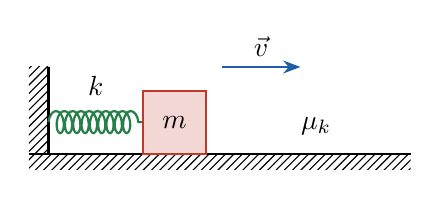
\begin{tikzpicture}[scale=1.0]
  \fill[pattern=north east lines] (-0.25,0) rectangle (0,1.1);
  \draw[thick] (0,0) -- (0,1.1);
  \fill[pattern=north east lines] (-0.25,-0.2) rectangle (4.6,0);
  \draw[thick] (-0.25,0) -- (4.6,0);
  \draw[decorate, decoration={coil, aspect=0.5, segment length=3pt, amplitude=4pt}, thick, verde] (0,0.4) -- node[above=6pt, text=black]{$k$} (1.2,0.4);
  \filldraw[draw=rojo, fill=rojo!20, thick] (1.2,0) rectangle (2.0,0.8);
  \node at (1.6,0.4) {$m$};
  \node at (3.4,0.35) {$\mu_k$};
  \draw[->, thick, azul] (2.2,1.1) -- node[above, text=black]{$\vec v$} (3.2,1.1);
\end{tikzpicture}
\end{document}
